%!TEX root = ../thesis.tex
\chapter{Applications \& Discussion}

This chapter presents a discussion of MapperGUI's software design and its consequences for musical mapping, as well as revisions made to the code since the initial release. The interface's features are explored in an attempt to evaluate the successes and failures of the design. Feedback from users was gathered throughout the project and through informal interviews after the software's release. This feedback is summarized and presented here. A modification to the code, motivated by feedback from users, is also described. MapperGUI is then compared to similar interfaces, analyzing especially for new features that could be incorporated into our flexible framework. Finally, the system is evaluated overall with respect to the project's initial goals.


%%%%%%%%%%%%%%%%%%%%%%%%%%%%%%%%%%%%%%%%%%%%%%%%%%%%%%%%%%%%%%%%%%%%%%%%%%%%%%%%%%%%%%%%%%%%%%%%%%%%%%%%%%%%%%%%%%%%%%%%%%%%%%%%%%%%%%%%%%%%%%%%%%%%%%%%%%%%%%%%%%%%%%%%%%%%%%%%%%%%%%%%%%%%%%%%%%%%%%%%%%%%%%%%%%%%%%%%%%%%%%%%%%%%%%%%%%%%%%%%%%%%%%%%%%%%%%%%%%
\section{User Feedback} % (fold)
\label{sec:user_feedback}

The entire MapperGUI project began with user feedback from prior GUIs for libmapper. Throughout the design process functional versions of MapperGUI were provided to libmapper users. Their feedback was crucially important to the evolution of the software. After the first official release of MapperGUI, long-term users were informally interviewed. These users were questioned specifically as to the projects with which utilized MapperGUI in an attempt to learn more concretely about the variety of use-cases for the software.

Even at this early stage of release, users have already incorporated MapperGUI into a wide variety of projects. This reflects our initial assumptions (based on experiences with prior GUIs) that a successful GUI must be flexible. Throughout development MapperGUI was used as an experimental tool and aid in designing DMIs. MapperGUI was used in concert with motion capture systems, vibrotactile feedback and even loaded onto a Raspberry PI\footnote{Raspberry Pi | An ARM GNU/Linux box for \$25. Take a byte! [Online] Available: \url{http://www.raspberrypi.org}. Accessed August 1, 2013}. During this whole process users encountered problems, had ideas for extensions and used the GUI in ways we could have never imagined.



%for response to vibrotactile feedback in a motion-capture study. It was also used in a motion capture setting for the design of an interactive audio installation. In the latter situation MapperGUI was required to handle many signals per single device, as each person in the room required 25 three-dimensional markers (75 signals total). A DMI designer has been using MapperGUI to test mappings for her input device with a single sound synthesizer, each containing about 30 signals.

%MapperGUI is being used as a development tool as well. A programmer is attempting to build a software bridge between libmapper and the Arduino\footnote{TODO}. She uses MapperGUI to test the robustness and effectiveness of the software, and has even successfully loaded the GUI onto a raspberryPI\footnote{TODO}

%\begin{table}
%\begin{center}
%\begin{tabular}{l p{5cm} p{5cm}}
	%\hline\hline
	%user&use case&concerns\\
	%\hline
	%Mailis&Intonespacio&saving and loading\\
	%Hakon&Experimenting with vibrotactile feedback and motion capture systems&Switching between various mappings\\
	%Clayton&An interactive space using motion capture&Reliability of network\\
	%Julie&libmapper code for firmata&Speed of function (she's using a rasperry Pi)\\
	%\hline
	%Andrew Stuart&teaches class with libmapper&\\
	%Gestes (Marlon)&Performance, etc.&Hide unconnected\\
%\end{tabular}
%\end{center}	
%\end{table}
%
%Hakon Knutzen, Mailis Rodrigues, Clayton Mamedes, Julie Ren\'e
		%%Mailis, Clayton, Hakon, Julie


	\subsection{General feedback} % (fold)
	\label{sub:general_feedback}

Most of our users had used libmapper previously, and had attempted to compile and use the library from scratch. Many commented on how well MapperGUI lowered the barriers to entry for non-technical users. Users who had never used libmapper before pointed out how much time had been saved in their work flow, versus when they used to hard-code mappings.

The best reviewed feature of MapperGUI was the automatic linear scaling control found in the top bar. Some users previously needed to detect signal minima and maxima by hand, then directly calculate and apply a linear scaling functions. With MapperGUI the task is trivially easy: one must simply enter the desired destination range and set the connection to the \emph{Calibrate} mode. Most of the ``magic'' in this feature is the result of the libmapper API, but providing users access through an easy-to-use GUI is also important. One user expressed frustration because she was not aware this feature existed, and instead continued to painstakingly condition her signals in Max/MSP. She was very impressed over how much time was saved by switching this workload to libmapper and MapperGUI.

Use of the other connection modes was rare. Users found the expression input box hard to use. Directly calculating the appropriate mathematical expression was seen as too abstract. This is a sensible problem to have, as difficult text-based input is precisely the thing that MapperGUI is designed to avoid. One user suggested a two-dimensional graphical tool, showing the transposition from input to output, to help with this task. 

Some users requested for signal values themselves to be available in MapperGUI. This would create a lot of bandwidth clutter, as all devices would need to constantly send signal data to the GUI. It was suggested the user should be able to query signal data by clicking or placing the mouse cursor over signal names.
	
	% subsection other_feedback (end)

	\subsection{Saving \& loading} % (fold)
	\label{sub:saving_and_loading}

Nearly all users made use of the saving and loading features in some way. For both experimental and design-based setups, returning to prior mappings is very useful, as it avoids the tedium of performing the same tasks repeatedly.

We received criticism for the na\"ive loading system. One user found it tedious that mappings would accumulate when loading multiple. He required rapid switching between the same few mappings for his experiment. Once these mappings were created there was little that needed to be done to modify them. For his experiment it became tedious to erase a previous mapping before loading a new one. Obviously in a live-performance context the amount of delay that would be created with this kind of task would be unacceptable. 

Another user wished to switch between mappings in his work, but required some kind of intermediate space between the states. Ideally loading would have the option of blending between two mappings, such that the transition is not too harsh for the audience. To maintain this functionality, the actual saving and loading of patches was transferred to Max/MSP for this project.

In a situation with many devices of the same class, loading a single mapping can be somewhat absurd. Because each connection will be loaded $m*n$ times, where $m$ is the number of similarly named input devices, and $n$ is the number of relevant output devices, certain simple mappings can result in hundreds of unwanted connections when a mapping is loaded. Perhaps some kind of staging area wherein the user must explicitly for which devices he or she wishes to load a mapping could solve this problem.

Another user asked for some kind of mapping preset that could be created and loaded whenever the program is opened. This way if the same experiment or performance is conducted repeatedly the user would simply need to launch MapperGUI and get started.
	
	% subsection saving_&_loading (end)

	\subsection{Reliability \& responsiveness} % (fold)
	\label{sub:reliability_and_responsiveness}

Multiple users commented on the frustrating nature of interacting with MapperGUI when it became out of sync with the libmapper network. As one user stated, ``The program is not useful if you do not \emph{trust} the display.'' In this way small errors, devices not appearing, signals not accepting connections, delays in operations, etc. become a very big problem for user satisfaction with MapperGUI. Users reviewed the refresh button very favorably. If something seemed amiss with the GUI or the network, and refreshing the display solved the problem, then trust in the display was restored.

Some problems were due to errors in the libmapper code and were out of the control of MapperGUI. Others were created when MapperGUI code started to make assumptions about the libmapper network. For example, with the drag-to-connect gesture, originally the drawn arrow persisted upon release of the mouse button. MapperGUI assumed that a connection would be made and kept the line to avoid delays. Of course, occasionally the signals were \emph{not} connected, due to dropped messages or incompatibility. In this circumstance the faulty arrow, representing nothing, became very confusing. Due to negative feedback the code was changed such that the drawn arrow disappears immediately after the drawing gesture. If the connection is successful, it is redrawn. This results in a slight flicker (as the arrow is erased and re-drawn), but this was much more popular than the potential erroneous arrows persisting in the display.

Some heavy operations, like scrolling and forming multiple connections, could create significant delays (on the order of a few seconds) in MapperGUI. Users responded very negatively to such delays, as they were accustomed to computer programs responding much more quickly. Generally multi-second delays were thought to be errors, thus reducing the user's trust in the application. In Section \ref{sec:testing_program_responsiveness} we explore solutions to this problem.
	
	% subsection reliability_and_responsiveness (end)

	\subsection{Effectiveness of alternate views} % (fold)
	\label{sub:effectiveness_of_alternate_views}

GridView and HiveView have only recently been recently included into the program. As a result most of our users are much more familiar with ListView. Users reported that while the alternate views were interesting, ListView was the most straightforward for creating mappings. It was reported that GridView was useful once most of the mapping was completed, as one could notice patterns that were not apparent in ListView, and alter mappings to reflect the findings. The limited functionality of HiveView meant that to most users it was simply a visualization tool. Also it was extremely common among our test users for use-cases to include very few devices with many connections, so the ``whole-network'' view in HiveView was not advantageous.
	
	% subsection effectiveness_of_alternate_views (end)
	
% section user_feedback (end)

%%%%%%%%%%%%%%%%%%%%%%%%%%%%%%%%%%%%%%%%%%%%%%%%%%%%%%%%%%%%%%%%%%%%%%%%%%%%%%%%%%%%%%%%%%%%%%%%%%%%%%%%%%%%%%%%%%%%%%%%%%%%%%%%%%%%%%%%%%%%%%%%%%%%%%%%%%%%%%%%%%%%%%%%%%%%%%%%%%%%%%%%%%%%%%%%%%%%%%%%%%%%%%%%%%%%%%%%%%%%%%%%%%%%%%%%%%%%%%%%%%%%%%%%%%%%%%%%%%
\section{Testing program responsiveness} % (fold)
\label{sec:testing_program_responsiveness}

Extension of interface features discussed in Section \ref{sec:extension_of_control_and_visual_elements} leads to some control possibilities that could be difficult for the GUI to handle. Addition of shortcut keys for connecting, linking, disconnecting and unlinking, as well as the ability to select multiple devices and signals at once allows users to create and delete hundreds of connections with a single key press. Na\"{i}ve saving and loading produces to situations where dense mappings will accidentally be applied to several instruments at once.

Though the ``update display'' model works extremely well for code modularity, it generates awkward situations when dealing with massive network operations. Since the system updates the entire display with each change to the network, deleting 100 links (if the user is clearing a large network) results in 100 independent \url{delete_link} messages arriving at the monitor. For each one of these messages, the display will fully update. In the case of ListView, all arrows will be cleared, and redrawn with one fewer present (as if the links are being deleted one-by-one). In total 4950 arrow drawing operations\footnote{$99 + 98 + 97 + ... + 2 + 1 = \frac{99*100}{2}$. Note that $\frac{n*(n+1)}{2}$ arrows will be drawn for any $n$ number of connections or links.} will occur, resulting in significant delay. 

As reported by users in Section \ref{sub:reliability_and_responsiveness}, any GUI operation that takes more than a few seconds, without some kind of visual feedback (like a ``loading'' bar), leads to frustration and mistrust of the program. Obviously, if the GUI is going to support these kinds of massive network manipulations, there needs to exist some way to keep them under control.

	\subsection{Rate limiting functions} % (fold)
	\label{sub:rate_limiting_certain_functions}

In order to prevent thousands of unnecessary, display re-draws, a ``waiting'' period was added to certain critical functions. This operating systems process is described in \shortciteN{os_concepts}. Essentially certain functions no longer execute in the code immediately once called, instead, a delay timer starts. If the function is called again during this delay, the delay timer simply restarts. The function is only executed once the delay timer finishes. This way, if a function is called 100 times simultaneously, it will only execute once after a short delay. Figure \ref{fig:waiting_period} shows the effect of the waiting period if the function is called a single time, and if it is called once during the delay.

\begin{figure}[ht]
	\centering
		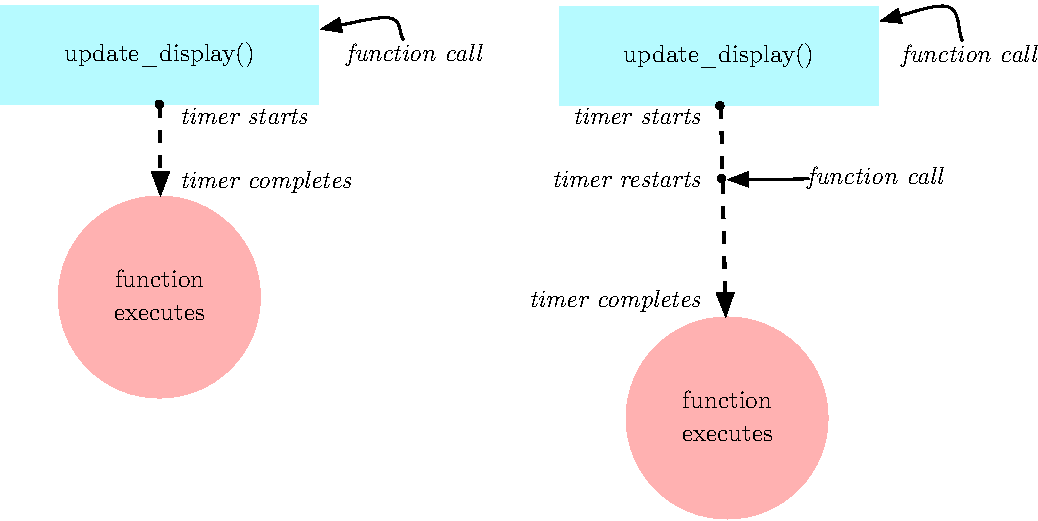
\includegraphics[width=1\textwidth]{figures/waiting_period}
		\caption{Illustration of a delayed function.}
		\label{fig:waiting_period}
\end{figure}

Two functions are limited in the GUI: \url{view.update_display} for all views and \url{update_arrows} for ListView. \url{update_display} is common to all views, and the massive network changes described above can result in many processor intesive functions to run needlessly. With the \url{update_arrows} function, operations that do not result in changes to the network (scrolling, changing tabs) require constant re-drawing.

Exactly how much time this delay should be set to is not obvious. If the delay is too short it is possible for massive network operations to still call the function many times if they arrive asynchronously. A too-long delay means that users may notice for simple actions, like scrolling with a single arrow (causing the scrolling to appear jerky). Another consequence of a long delay is that a process which calls the delayed function at a regular interval could continuously restart the delay. In this case the function will \emph{never} execute, a situation known as ``starvation'' \shortcite{os_concepts}.

After some informal tests of delays between 17 and 1000 milliseconds, a delay of 33 milliseconds was selected for both functions. Substantial improvement in execution speed was observed for even very short delays, as often hundreds of function calls would reach the \url{view.update_display} virtually simultaneously. With delays closer to one second there was little improvement in response to massive network operations, and the delay itself became noticeable (especially with scrolling operations). 33 milliseconds is in the range where nearly every operation results in just a single function being executed, but is also an imperceptible delay to a human user. The number 33 itself was selected because it is the length of two screen refreshes on a 60 Hz display (a measure recommended in \shortciteNP{os_concepts}).
	
	% subsection rate_limiting_certain_functions (end)

% section testing_program_responsiveness (end)

%%%%%%%%%%%%%%%%%%%%%%%%%%%%%%%%%%%%%%%%%%%%%%%%%%%%%%%%%%%%%%%%%%%%%%%%%%%%%%%%%%%%%%%%%%%%%%%%%%%%%%%%%%%%%%%%%%%%%%%%%%%%%%%%%%%%%%%%%%%%%%%%%%%%%%%%%%%%%%%%%%%%%%%%%%%%%%%%%%%%%%%%%%%%%%%%%%%%%%%%%%%%%%%%%%%%%%%%%%%%%%%%%%%%%%%%%%%%%%%%%%%%%%%%%%%%%%%%%%
\section{Comparison to Similar Interfaces} % (fold)
\label{sec:comparison_to_similar_interfaces}

Other systems exist to help non-programmers map control inputs to sound synthesis parameters. This section compares this research to these related works.

\begin{figure}
	\centering
		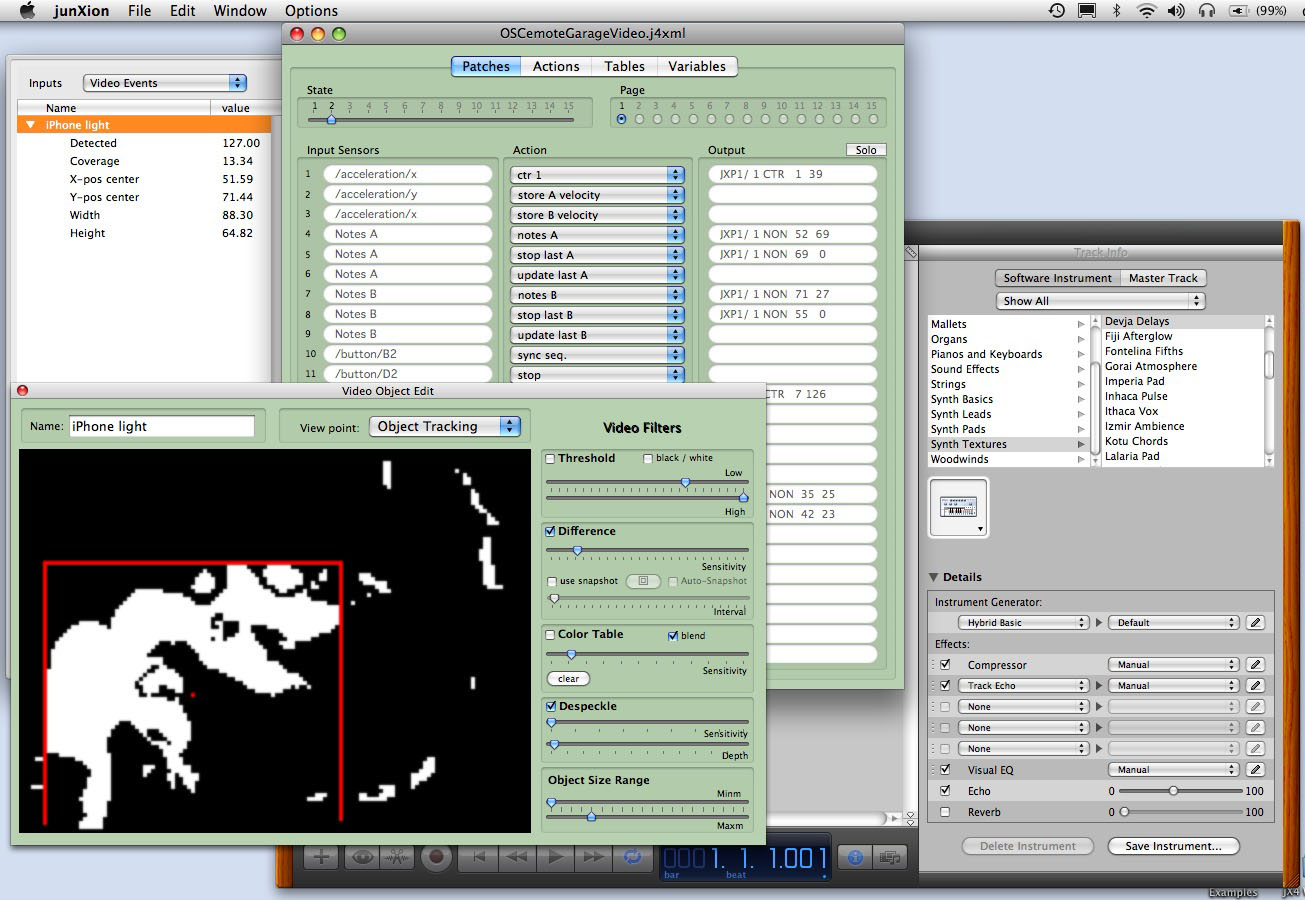
\includegraphics[width=\textwidth]{figures/junXion_v4}
		\caption{STEIM's JunXion software}
		\label{fig:junxion}
\end{figure}

The Studio for Electro-Instrumental Music (STEIM) distributes JunXion \cite{junxion}, a software application for controlling MIDI and OSC-based systems. JunXion automatically detects input devices like computer mice and USB video-game controllers. The user is able to drag any child signals from these controllers onto one of 25 possible inputs.  From there the user can switch to the ``actions'' tab, where destinations and connection properties can be customized. Connection properties are stored in groups that populate drop-down menus in the central column. JunXion features a very interesting ``state'' system similar to MapperGUI's saving and loading. Once a successful mapping is created, users can change the state, starting a new mapping. With multiple mappings, users can quickly switch between states. JunXion also has a very interesting graphical signal conditioning editor. The program presents a two dimensional field and the user can draw, generate curves and set bounds. Incorporating such a feature into MapperGUI would assist users who were unimpressed by textual expression input.

\begin{figure}
	\centering
		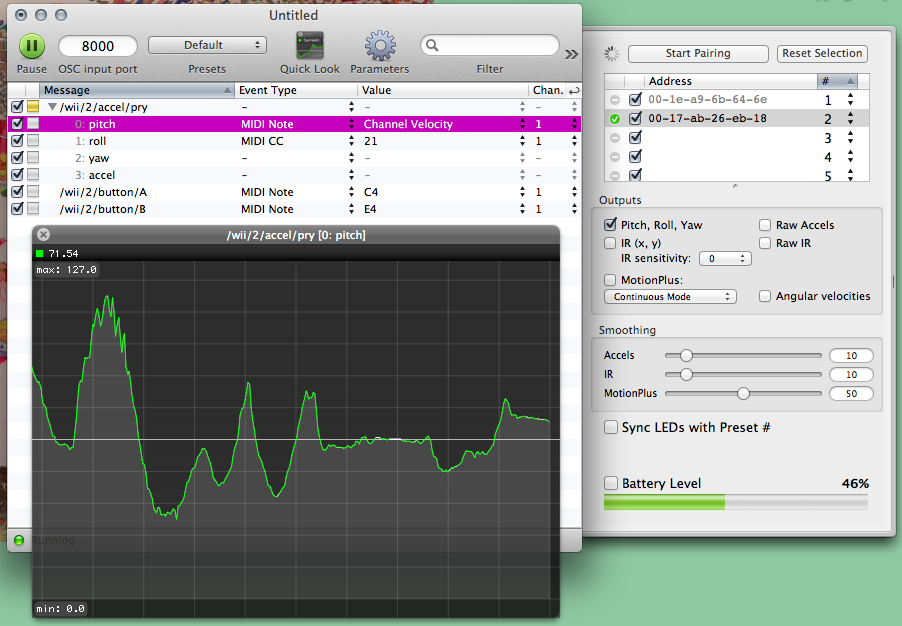
\includegraphics[width=\textwidth]{figures/osculator}
		\caption{The OSCulator interface}
		\label{fig:osculator}
\end{figure}

The OSCulator system \cite{osculator} is very similar to JunXion. Compatible controllers appear automatically and can be mapped to MIDI or OSC signals. OSCulator also relies on a drop-down menu based interface for selecting where and how the output will be routed. As in JunXion the idea of a ``connection'' is not emphasized, instead a MIDI or OSC message is simply sent on a specific channel (the receiving end must be specifically notified on which channel to receive messages). As can be seen in Figure \ref{fig:osculator}, OSCulator displays a real-time oscilloscope like visualization for selected signals. A similar feature would help MapperGUI with visual feedback, which was a desire of some users.

The Eaganmatrix \cite{eaganmatrix} partly inspired GridView in MapperGUI. The signals of a single control and synthesis device are displayed on the x and y axes of a grid display. Connections between the two are made by clicking on the intersections. The Patchage interface \cite{patchage} contains uses an interaction very similar to ListView, where objects containing lists of signals can be connected by dragging gestures. Max/MSP and an Integra Live \cite{integra} also feature this interaction, but neither are necessarily for creating mappings. 

	% subsection other_similar_interfaces (end)

% section comparison_to_similar_interfaces (end)




